%
% FH Technikum Wien
% !TEX encoding = UTF-8 Unicode
%
% Erstellung von Master- und Bachelorarbeiten an der FH Technikum Wien mit Hilfe von LaTeX und der Klasse TWBOOK
%
% Um ein eigenes Dokument zu erstellen, müssen Sie folgendes ergänzen:
% 1) Mit \documentclass[..] einstellen: Master- oder Bachelorarbeit, Studiengang und Sprache
% 2) Mit \newcommand{\FHTWCitationType}.. Zitierstandard festlegen (wird in der Regel vom Studiengang vorgegeben - bitte erfragen)
% 3) Deckblatt, Kurzfassung, etc. ausfüllen
% 4) und die Arbeit schreiben (die verwendeten Literaturquellen in Literatur.bib eintragen)
%
% Getestet mit TeXstudio mit Zeichenkodierung ISO-8859-1 (=ansinew/latin1) und MikTex unter Windows
% Zu beachten ist, dass die Kodierung der Datei mit der Kodierung des paketes inputenc zusammen passt!
% Die Kodierung der Datei twbook.cls MUSS ANSI betragen!
% Bei der Verwendung von UTF8 muss dnicht nur die Kodierung des Dokuments auf UTF8 gestellt sein, sondern auch die des BibTex-Files!
%
% Bugreports und Feedback bitte per E-Mail an latex@technikum-wien.at
%
% Versionen
% *) V0.7: 9.1.2015, RO: Modeline angepasst und verschoben
% *) V0.6: 10.10.2014, RO: Weitere Anpassung an die UK
% *) V0.5: 8.8.2014, WK: Literaturquellen überarbeitet und angepasst
% *) V0.4: 4.8.2014, WK: Initalversion in SVN eingespielt
%
\documentclass[MMR,Master,english]{twbook}
\usepackage[utf8]{inputenc}
\usepackage[T1]{fontenc}
%
% Hier biblatex & Biber konfigurieren; Vergessen Sie nicht, dass Sie biber verwenden müssen um eine Bibliothek zu erzeugen
%
\usepackage[backend=biber, style=numeric]{biblatex}
\addbibresource{Literatur.bib}

%
% Bei Bedarf bitte hier die Syntax-Highlightings anpassen
%
\usepackage{float}
\usepackage{comment}
\usepackage{csquotes}
%
% Platzierungsoptionen 
%
\usepackage[final]{listings}
\lstset{captionpos=b, numberbychapter=false,caption=\lstname,frame=single, numbers=left, stepnumber=1, numbersep=2pt, xleftmargin=15pt, framexleftmargin=15pt, numberstyle=\tiny, tabsize=3, columns=fixed, basicstyle={\fontfamily{pcr}\selectfont\footnotesize}, keywordstyle=\bfseries, commentstyle={\color[gray]{0.33}\itshape}, stringstyle=\color[gray]{0.25}, breaklines, breakatwhitespace, breakautoindent}
\lstloadlanguages{[ANSI]C, C++, [gnu]make, gnuplot, Matlab}

%Formatieren des Quellcodeverzeichnisses
\makeatletter
% Setzen der Bezeichnungen für das Quellcodeverzeichnis/Abkürzungsverzeichnis in Abhängigkeit von der eingestellten Sprache
\providecommand\listacroname{}
\@ifclasswith{twbook}{english}
{%
    \renewcommand\lstlistingname{Code}
    \renewcommand\lstlistlistingname{List of Code}
    \renewcommand\listacroname{List of Abbreviations}
}{%
    \renewcommand\lstlistingname{Quellcode}
    \renewcommand\lstlistlistingname{Quellcodeverzeichnis}
    \renewcommand\listacroname{Abkürzungsverzeichnis}
}
% Wenn die Option listof=entryprefix gewählt wurde, Definition des Entyprefixes für das Quellcodeverzeichnis. Definition des Macros listoflolentryname analog zu listoflofentryname und listoflotentryname der KOMA-Klasse
\@ifclasswith{scrbook}{listof=entryprefix}
{%
    \newcommand\listoflolentryname\lstlistingname
}{%
}
\makeatother
\newcommand{\listofcode}{\phantomsection\lstlistoflistings}

% Die nachfolgenden Pakete stellen sonst nicht benötigte Features zur Verfügung
\usepackage{blindtext}

%
% Einträge für Deckblatt, Kurzfassung, etc.
%
\title{Virtualisierung eines Echtzeit-Betriebssystems zur Steuerung eines Roboters mit Schwerpunkt auf die
Einhaltung der Echtzeit}
\author{Halil Pamuk, BSc}
\studentnumber{51842568}
%\author{Titel Vorname Name, Titel\and{}Titel Vorname Name, Titel}
%\studentnumber{XXXXXXXXXXXXXXX\and{}XXXXXXXXXXXXXXX}
\supervisor{Sebastian Rauh, MSc. BEng}
%\supervisor[Begutachter]{Titel Vorname Name, Titel}
%\supervisor[Begutachterin]{Titel Vorname Name, Titel}
%\secondsupervisor{Titel Vorname Name, Titel}
%\secondsupervisor[Begutachter]{Titel Vorname Name, Titel}
%\secondsupervisor[Begutachterinnen]{Titel Vorname Name, Titel}
\place{Wien}
\kurzfassung{Erstellung einer Echtzeit-Robotersteuerungsplattform unter Verwendung von Salamander OS, Xenomai, QEMU
und PCV-521 in der Yocto-Umgebung. Die Plattform basiert auf Salamander OS und nutzt Xenomai für Echtzeit-
Funktionen. Dazu muss im ersten Schritt die Virtualisierungsplattform evaluiert werden. (QEMU, Hyper-V, Virtual
Box, etc.) Als weiterer Schritt folgt die Anbindung eines Roboters über eine VARAN-Bus Schnittstelle. Das
gesamte System wird in der Yocto-Umgebung erstellt und konfiguriert.
Das Hauptziel der Arbeit ist es, herauszufinden, wie die Integration von Echtzeit-Funktionen und effizienten
Kommunikationssystemen in eine Robotersteuerungsplattform die Reaktionszeit und Zuverlässigkeit von
Roboteranwendungen verbessern kann}
\schlagworte{Schlagwort1, Schlagwort2, Schlagwort3, Schlagwort4}
\outline{Abstract}
\keywords{Echtzeit, Virtualisierung, Xenomai, VARAN}
%\acknowledgements{\blindtext}

\begin{document}

\maketitle

%
% .. und hier beginnt die eigentliche Arbeit. Viel Erfolg beim Verfassen!
%
%Die folgende Gliederung von Bachelor- und Masterarbeiten ist für die Robotik-Studiengänge
%verpflichtend vorgeschrieben.
%
%- Deckblatt
%- Eidesstattliche Erklärung (digital signiert)
%- Kurzfassung und Abstract mit Schlüsselwörtern/Keywords
%- Danksagung (optional)
%- Inhaltsverzeichnis

%- Einleitung (die genannten Punkte müssen keine eigenen Unterkapitel sein, müssen aber aus der Einleitung klar hervorkommen):
%   - Stand der Technik
%   - Problem- und Aufgabenstellung
%   - Zielsetzung
%- Hauptteil -> Gliederung je nach Thema
%   - Methodik
%   - Resultate
%   - Wirtschaftliche Betrachtung (optional)
%   - Diskussion
%- Zusammenfassung und Ausblick

%- Literaturverzeichnis
%- Abbildungsverzeichnis
%- Tabellenverzeichnis
%- Abkürzungsverzeichnis (optional)
%- Glossar (optional)
%- Anhang (optional)
\chapter{Introduction}
In today's industrial production and automation, robot systems are well established and of crucial importance. Robots must react to their environment and perform time-critical tasks within strict time constraints. Delays or errors can have catastrophic consequences in some cases. Traditional operating systems, such as Windows or Linux, are often not suitable for these types of real-time requirements as they cannot guarantee deterministic execution times. Therefore, real-time operating systems are required that are specifically designed to react to events within fixed time limits and prioritise the execution of high-priority processes. 

\bigskip \noindent The core component of an RTOS that enables real-time capabilities is the kernel. The kernel is responsible for managing system resources, scheduling tasks, and ensuring deterministic behavior. It employs preemptive scheduling mechanisms to allow high-priority tasks to preempt lower-priority tasks, ensuring that time-critical tasks are not delayed. The kernel also implements priority-based scheduling algorithms, such as Rate Monotonic Scheduling (RMS) or Earliest Deadline First (EDF), to schedule tasks based on their priorities and timing constraints. Additionally, RTOS kernels are designed to minimize interrupt latency, which is crucial for real-time applications that require immediate response to external events.

\bigskip \noindent In these RTOS systems, task scheduling is based on so-called priority-based preemptive scheduling. Each task in a software application is assigned a priority. A higher priority means that a faster response is required. Pre-emptive task scheduling ensures a very fast response. Preemptive means that the scheduler can stop a currently running task at any point if it recognises that another task needs to be executed immediately. The basic rule on which priority-based preemptive scheduling is based is that the task with the highest priority that is ready to run is always the task that must be executed. So if both a task with a lower priority and a task with a higher priority are ready to run, the scheduler ensures that the task with the higher priority runs first. The lower priority task is only executed once the higher priority task has been processed. Real-time systems are usually categorised as either soft or hard real-time systems. The difference lies exclusively in the consequences of a violation of the time limits. 

\bigskip \noindent Hard real-time is when the system stops operating if a deadline is missed, which can have catastrophic consequences. These consequences include endangering people, damaging machinery, impacting the health and integrity of the environment. Typical examples of this are some control systems in aeroplanes or cars, e.g. internal combustion engines.

\bigskip \noindent Soft real-time exists when a system continues to function even if it cannot perform the tasks within a specified time. If the system has missed the deadline, this has no critical consequences. The system continues to run, although it does so with undesirably lower output quality. Examples of this are multimedia systems where the occasional deviation from a playback rate of 25 frames/sec. leads to stuttering or similar.


%In der heutigen industriellen Fertigung und Automatisierung sind Robotersysteme sehr etabliert und von entscheidender Bedeutung. Roboter müssen auf ihre Umgebung reagieren und zeitkritische Aufgaben innerhalb strenger Zeitvorgaben ausführen. Verzögerungen oder Fehler können in einigen Fällen katastrophale Konseqenzen haben. Traditionelle Betriebssysteme, wie Windows oder Linux sind für diese Art von Echtzeitanforderungen oft nicht geeignet, da sie keine deterministischen Ausführungszeiten garantieren können. Daher sind Echtzeit-Betriebssysteme nötig, die speziell dafür konzipiert sind, auf Ereignisse innerhalb fester Zeitschranken zu reagieren und Prozesse mit hoher Priorität bevorzugt auszuführen. Bei diesen RTOS-Systemen basiert das Task-Scheduling auf dem sogenannten prioritätsbasierten präemptiven Scheduling. Jeder Task in einer Software-Applikation ist eine Priorität zuzuweisen. Eine höhere Priorität bedeutet, dass eine schnellere Reaktion erforderlich ist. Durch das präemptive Task-Scheduling wird eine sehr schnelle Reaktion sichergestellt. Präemptiv bedeutet, dass der Scheduler eine gerade laufende Task an jeder Stelle anhalten kann, wenn er erkennt, dass eine andere Task sofort ausgeführt werden muss. Die Grundregel, auf der das prioritätsbasierte präemptive Scheduling basiert, besagt, dass die ausführbereite Task mit der höchsten Priorität immer die Task ist, die ausgeführt werden muss. Wenn also sowohl eine Task mit niedriger als auch eine Task mit höherer Priorität ausführbereit sind, sorgt der Scheduler dafür, dass zuerst die Task mit der höheren Priorität läuft. Die Task mit niedrigerer Priorität wird erst dann ausgeführt, wenn die höherpriore Task verarbeitet wurde.

%\noindent Echtzeitsysteme werden in der Regel entweder als weiches oder als hartes Echtzeitsystem kategorisiert. Der Unterschied liegt ausschließlich in den Folgen einer Verletzung der Zeitschranken.

%\noindent Harte Echtzeit liegt vor, wenn das System seinen Betrieb einstellt, wenn ein Termin verpasst wurde, was katastrophale Folgen haben kann. Zu diesen Folgen zählen die Gefährdung von Menschen, die Beschädigung von Maschinen, also Auswirkungen auf Gesundheit und Unversehrtheit der Umgebung. Typische Beispiele hierfür sind einige Steuerungssysteme im Flugzeug oder im Auto, z.B. bei der Verbrennungsmaschine.

%\noindent Weiche Echtzeit besteht, wenn ein System weiter funktionsbereit ist, selbst wenn es die Aufgaben innerhalb einer festgelegten Zeit nicht ausführen kann. Wenn das System den Termin verpasst hat, hat dies keine kritischen Konsequenzen. Das System läuft weiter, obwohl es dies mit unerwünscht geringerer Ausgabenqualität tut. Beispiele hierfür sind Multimediasysteme, bei denen das gelegentlich Abweichen von einer Abspielrate von 25 Bildern/sek. zu einem Ruckeln o.ä. führt.



\clearpage
\section{Thesis Context}
Diese Masterarbeit wurde in der Firma SIGMATEK GmbH \& Co KG erstellt. 





\clearpage
\section{State of the art}







\clearpage


\section{Problem and task definition}
In robotics, accurate and timely control is crucial to ensure precise movements and reliable interaction with the environment. However, existing robot control systems often have limitations in terms of real-time capabilities and communication efficiency, which can have a detrimental effect on response time and reliability. The challenge is to develop a powerful real-time robot control platform that overcomes these limitations and improves the performance of robotic applications.


\clearpage
\section{Objective}

The main objective of this work is to create a real-time robot control platform that integrates Salamander OS, Xenomai, QEMU and PCV-521 in the Yocto environment. 

This integration is expected to lead to a significant improvement in the response time and reliability of robot applications.


%%%%%%%%%%%%%%%%%%%%%%%%%%%%%%%%%%%%%%%%%%%%%%%%%%%%%%%%%%
\clearpage
\chapter{Methodology}
 
In diesem Abschnitt werden sämtliche theoretischen Konzepte und Randbedingungen sowie praktische Methoden, die zur Erreichung der Zielsetzung dieser Masterarbeit beigetragen haben, detailliert beschrieben.

Zu Beginn der Arbeit wurde eine ausführliche Analyse der einzelnen Virtualisierungsmöglichkeiten von Salamander 4 durchgeführt. Im Besonderen wurde hier die Virtualisierungsperformance von Ubuntu 22.04, Windows 10 und WSL unter QEMU verglichen.

First, a comprehensive literature review is conducted to understand the current trends and challenges in real-time robot control. Based on the literature study, a suitable virtualisation platform is selected. 


After the selection of the virtualisation platform, the robot control platform is implemented. This step includes the installation and configuration of Salamander OS, Xenomai, QEMU and PCV-521 in the Yocto environment. Once the platform has been implemented, the robot is connected via a VARAN bus interface. Finally, the platform is evaluated to determine how the integration of real-time functions and efficient communication systems improves the response time and reliability of robot applications.

- Evaluation der Virtualisierungsplattform: 
Ich werde verschiedene Virtualisierungsplattformen wie QEMU, Hyper-V, Virtual Box usw. evaluieren. Dies ist ein wichtiger Schritt, um die beste Plattform für meine Anforderungen zu finden.
  
- Erstellung und Konfiguration des Systems in der Yocto-Umgebung: 
Ich werde das Yocto-Framework verwenden, um mein Embedded Linux System zu erstellen und zu konfigurieren. Yocto bietet viele Tools und Funktionen, die mir bei der Erstellung und Konfiguration meines Systems helfen können.

- Verbesserung der Reaktionszeit und Zuverlässigkeit von Roboteranwendungen: 
Mein Hauptziel ist es, herauszufinden, wie die Integration von Echtzeitfunktionen und effizienten Kommunikationssystemen die Reaktionszeit und Zuverlässigkeit von Roboteranwendungen verbessern kann. Ich strebe an, die Leistung und Zuverlässigkeit meiner Roboteranwendungen zu verbessern, indem ich ihre Fähigkeit verbessere, in Echtzeit auf Ereignisse zu reagieren.

- Anbindung eines Roboters über eine VARAN-Bus Schnittstelle:
Ich plane, einen Roboter in mein System zu integrieren. Ich werde eine VARAN-Bus Schnittstelle verwenden, um eine schnelle und zuverlässige Kommunikation zwischen dem Roboter und dem Steuerungssystem zu gewährleisten.

\bigskip \noindent Trace-cmd was used for tracing the Linux kernel. It can record various kernel events such as interrupts, scheduler decisions, file system activity, function calls in real time. Trace-cmd helped in getting detailed insights into system behaviour and identify reasons for latency \cite{Tracecmd}. 

\bigskip \noindent The data that was recorded by trace-cmd was then fed into Kernelshark, which is a graphical front-end tool. It visualizes the recorded kernel trace data in a readable way on an interactive timeline, which facilitated the process of identifying patterns and correlations between events. By further filtering the displayed events according to specific criteria such as processes, event types or time ranges, the latency issues were analyzed \cite{KernelShark}. 

\bigskip \noindent Real-time operating system capabilities were provided by Xenomai, which is real-time development framework that extends the Linux kernel. It enables low-latency and deterministic execution of time-critical tasks. Xenomai introduces a dual-kernel approach with a real-time kernel coexisting alongside Linux. A key utility within the Xenomai suite is the latency tool, which benchmarks the timer latency - the time it takes for the kernel to respond to timer interrupts or task activations. The tool creates real-time tasks or interrupt handlers and measures the latency between expected and actual execution times\cite{Xenomai}.


\clearpage 
\chapter{Salamander Operating System}
Salamander 4 ist das proprietäre Betriebssystem.
Es basiert auf der der Linux-Version 5.15.94 und integriert zusätzlich Xenomai 3.2, eine Echtzeit-Entwicklungsumgebung \cite{Xenomai}. Es handelt sich um ein 64-Bit-System, was auf die x86\_64-Architektur hinweist. Das Echtzeitverhalten wird durch die Verwendung von Symmetric Multi-Processing (SMP) und Preemptive Scheduling (PREEMPT) erreicht. Darüber hinaus nutzt es IRQPIPE, um Interrupts in einer Weise zu verarbeiten, die die Echtzeitanforderungen des Systems erfüllt. Xenomai besteht aus 3 Teilen. Diese sind der Tabelle \ref{tab:what_is_xenomai} zu entnehmen 

\begin{table}[!h]
    \centering
    \caption[Kurz]{Lang}
    \label{tab:what_is_xenomai}
    \setlength{\tabcolsep}{0.5em} % for the horizontal padding
    {\renewcommand{\arraystretch}{1.2}% for the vertical padding
    \begin{tabular}{|c|p{0.6\textwidth}|}
        \hline
        \textbf{Teil} & \textbf{Beschreibung} \\ \hline
        i-pipe  & Kernelerweiterung für das Domain-Konzept \\ \hline
        Xenomai Kernel & Benutzt die i-pipe, und hängt sich als root-Domain ein \\ \hline
        Xenomai User &  Programme (LRT) verwenden diese Bibliothek, um Xenomai Funktionen verwenden zu können. \\ \hline
    \end{tabular}}
  \end{table}
  

\noindent Xenomai beruht auf einem Domain-Konzept, das bedeutet, dass alle IRQ an die erste Domain gesendet werden. (root – Domain / Xenomai)
Nur wenn diese nichts mehr zu tun hat, dann darf die 2. Domain arbeiten.
Das bedeutet, erst wenn alle Xenomai Task in einem Wartezustand sind, arbeiten die Linux-Tasks.

\noindent In der Regel unterbricht der Prozessor beim IRQ-Handling seine aktuellen Aktivitäten, um einen Interrupt zu bearbeiten, während die IRQ-Behandlung von Xenomai einen Interrupt-Pipeline-Mechanismus verwendet, der das gleichzeitige Abrufen und Vorbereiten eines anderen Interrupts ermöglicht, während ein Interrupt bearbeitet wird, was die Leistung verbessert und die Latenzzeit verringert.  

\noindent Was Xenomai4 von seinem Vorgänger Xenomai3 unterscheidet, ist die vollständige Neugestaltung der Ausführungsphase mit hoher Priorität. Dies geschah aus Gründen der Portabilität und Wartungsfreundlichkeit: I-pipe - die zweite Iteration der ursprünglichen Adeos-Interrupt-Pipeline - wurde vollständig durch Dovetail ersetzt. 

\begin{table}[H]
    \centering
    \caption[Kurz]{Lang}
    \label{tab:domain_specific_functions}
    \begin{tabular}{|c|c|}
        \hline
        \textbf{Xenomai spezifische Funktionen} & \textbf{Linux spezifische Funktionen} \\ \hline
        Tasks                                   & Dateizugriffe                           \\ \hline
        Mutexes, Semaphoren, Events             & Netzwerk                                \\ \hline
    \end{tabular}
\end{table}


\noindent Ein Aufruf dieser Funktionen erfordert die entsprechende Domain. Wenn der Task in der falschen Domain läuft, dann wird ein Domain-Wechsel forciert.
Ein Domainwechsel von Xenomai nach Linux geht relativ einfach. Aber der Wechsel von Linux nach Xenomai braucht Unterstützung, und dafür ist die Hilfe des Gatekeepers notwendig. Das bedeutet, der Gatekeeper hilft einem Task von Linux nach Xenomai zu wechseln.

\section{Task priorities}
Es gibt grundsätzlich 4 Gruppen

\begin{table}[ht]
    \centering
    \caption{Übersicht der Prioritätsgruppen und ihrer Beziehungen}
    \label{tab:priorities}
    \begin{tabular}{|c|c|}
        \hline
        \textbf{Prioritätsgruppe} & \textbf{Bereich}  \\ \hline
        Xenomai Priorität & 0 bis 99  \\ \hline
        Linux RT Priorität & 1 bis 99 \\ \hline
        Linux (Nice Level) Priorität & -20 bis 19  \\ \hline
        RTK Priorität & 0 bis 14 \\ \hline
    \end{tabular}

\end{table}
 



\section{Memory Management}
Es gibt verschiedene Speicherbereiche

Linux/System/Programm Speicher
	Der Speicher, den Linux und Programme belegt haben.
	Dieser Speicher ist intern in viele Teile aufgeteilt. (DMA, …)

LRT-Heap Speicher
	Speicher den der LRT verwendet, oder welcher über ein CIL Funktionen
	angefordert wird.

App Heap, App Code, …


\begin{figure}[H]
    \centering
    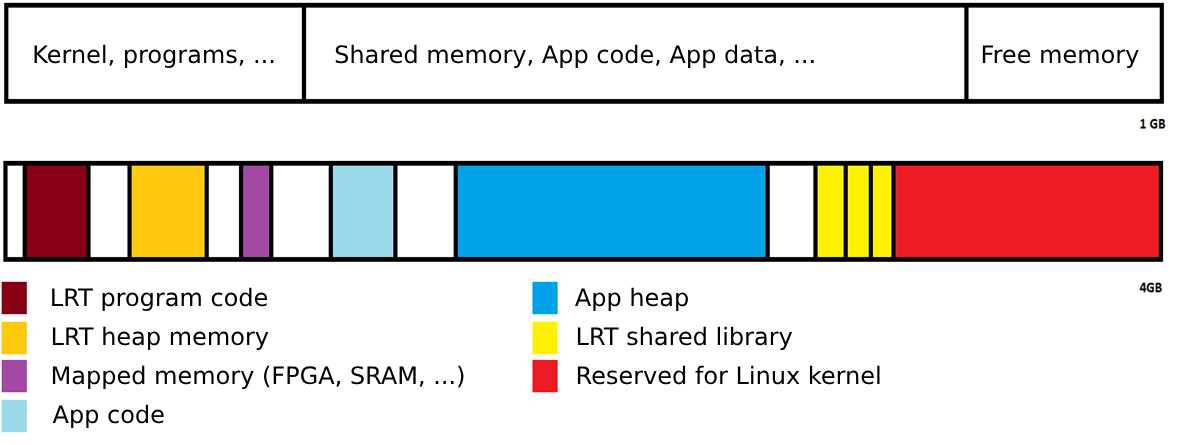
\includegraphics[width=0.8\columnwidth]{img/RAM_Memory_management.png}
    \caption[Kurz]{Lang}
    \label{fig:memory_management}
  \end{figure}


  Eine LASAL CPU besteht aus den folgenden Software-Modulen:
  \begin{itemize}
    \item Operating system
    \item Loader
    \item Hardware-Klassen
  \end{itemize}
  
  Die Schnittstelle zwischen den einzelnen Modulen wird in Abbildung \ref{fig:lasal_cpu} durch einen Pfeil gekennzeichnet.

  \begin{figure}[!h]
    \centering
    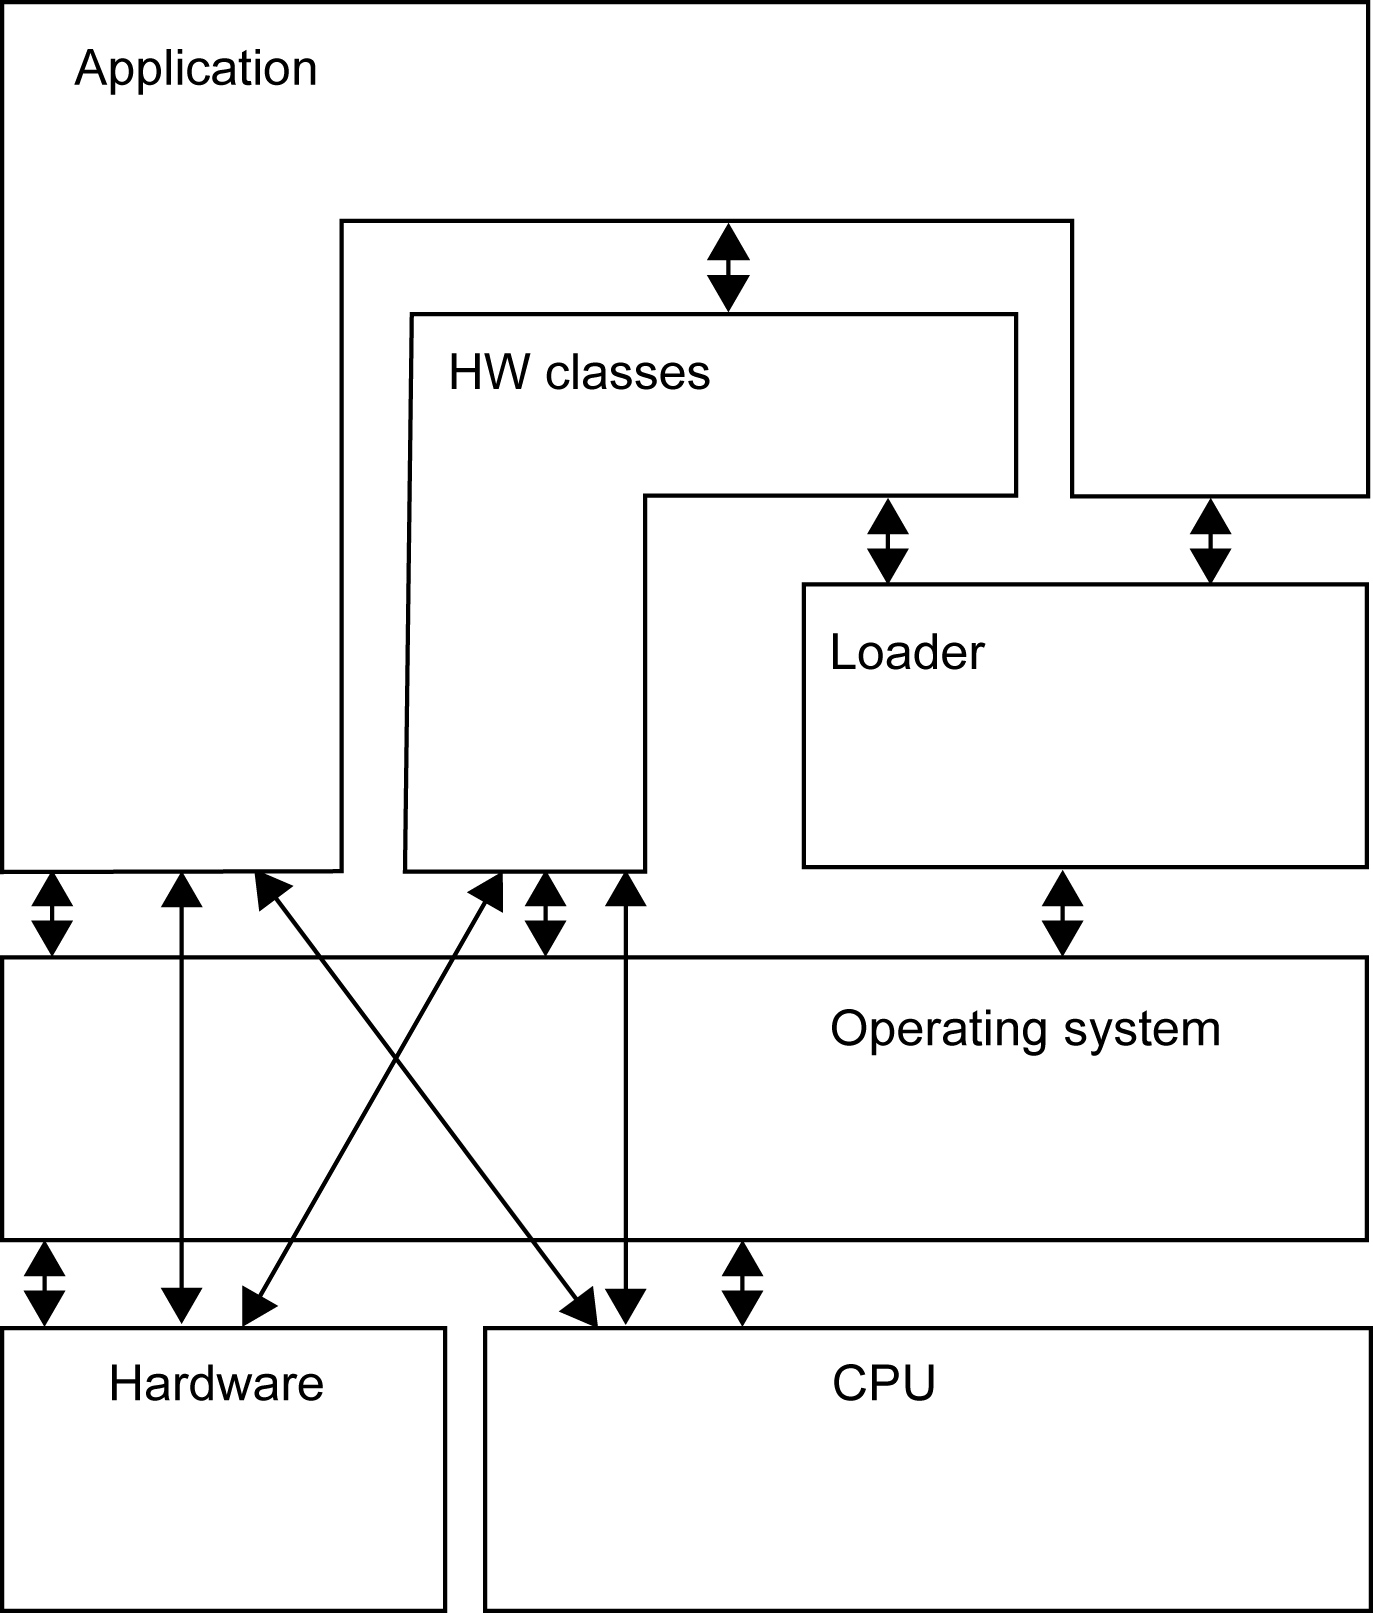
\includegraphics[width=0.5\columnwidth]{img/Software-Struktur einer LASAL CPU.png}
    \caption[Kurz]{Lang}
    \label{fig:lasal_cpu}
  \end{figure}

\clearpage


\chapter{Comparison of Real-Time Latency}

\section{Salamander 4 Bare Metal}




\section{Salamander 4 Virtualisation}




Salamander 4 





\section{Kernelshark}




\chapter{Results}
Firma SIGMATEK\newline
Yocto\newline
Salamander 4\newline
Xenomai\newline
QEMU\newline
Trace-cmd\newline
Kernelshark\newline
VARAN-Bus PCV-521\newline
Windows\newline
Ubuntu\newline
WSL\newline
\clearpage
\chapter{Discussion}
\clearpage
\chapter{Summary and Outlook}

%
% Hier beginnen die Verzeichnisse.
%
\clearpage
\printbibliography
\clearpage

% Das Abbildungsverzeichnis
\listoffigures
\clearpage

% Das Tabellenverzeichnis
\listoftables
\clearpage

% Das Quellcodeverzeichnis
\listofcode
\clearpage

\phantomsection
\addcontentsline{toc}{chapter}{\listacroname}
\chapter*{\listacroname}
\begin{acronym}[XXXXX]
    \acro{ABC}[ABC]{Alphabet}
    \acro{WWW}[WWW]{world wide web}
    \acro{ROFL}[ROFL]{Rolling on floor laughing}
\end{acronym}

%
% Hier beginnt der Anhang.
%
\clearpage
\appendix
\chapter{Anhang A}
\clearpage
\chapter{Anhang B}
\end{document}
